
% =======================
% Capa Estilo Tanenbaum
% =======================
\newcommand{\makecapa}{
  \begin{titlepage}
    \thispagestyle{empty}

    \begin{tikzpicture}[remember picture, overlay]
% Faixa Superior (Topo)
\fill[verdeuni]
(current page.north west)
rectangle ++(\paperwidth,-6.5cm);


      
      % Texto do Topo: Autores e Título Principal
      \node[anchor=north, text width=\paperwidth, align=center] at ([yshift=-1.5cm]current page.north) {
        {\Large\sffamily\color{white}  SERGIO S. NOVAK, LEANDRO M. P. SANCHES, RONALDO CAMILO DOS SANTOS } \\[0.8cm]
        {\Huge\bfseries\sffamily\color{yellow} Banco de Dados} \\[0.4cm]
        {\Large\sffamily\color{white} 1ª EDIÇÃO}
      };

      % Imagem Central (A ilustração de commodities que geramos)
      % Ela fica posicionada entre as faixas, como no livro original
      \node[anchor=center] at ([yshift=-2.2cm]current page.center) {
        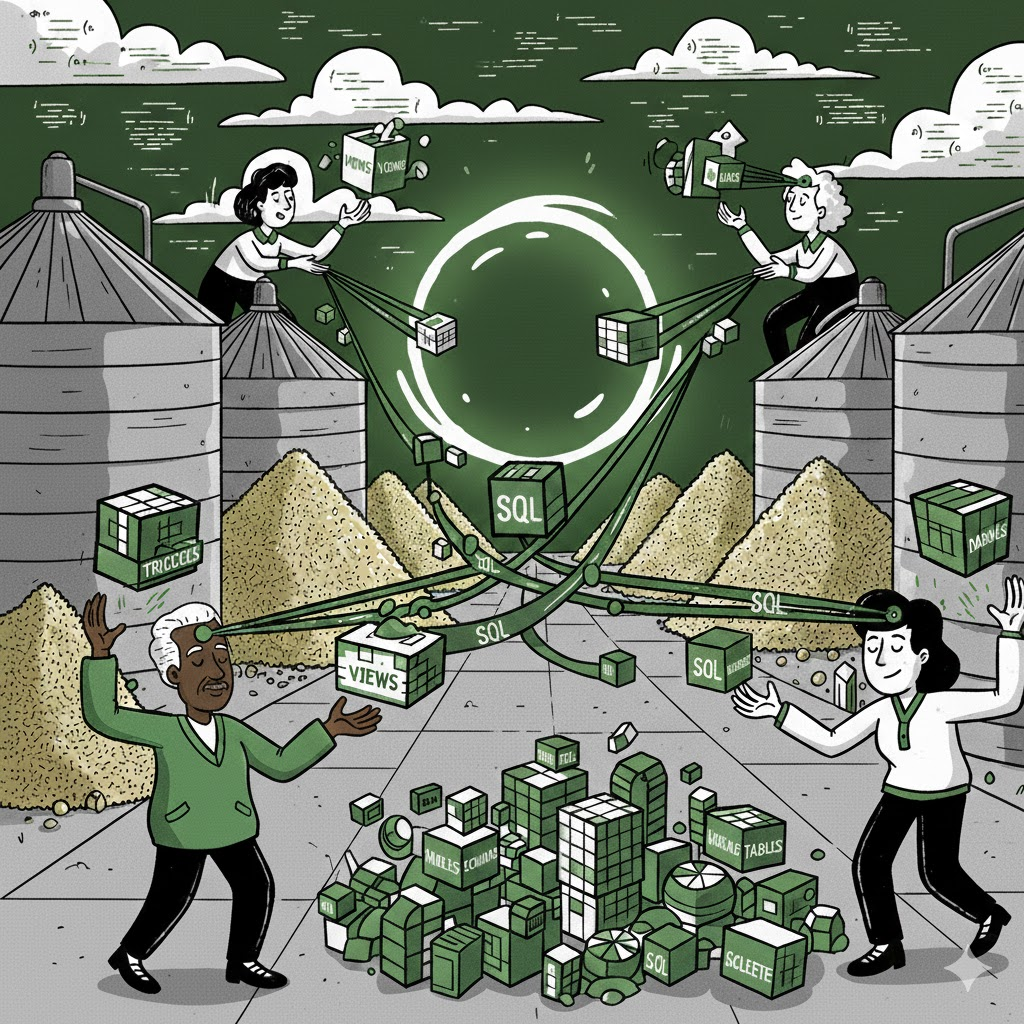
\includegraphics[width=1.02\paperwidth]{capa.jpg} % Ligeiramente maior para sangria lateral
      };

      % Faixa Inferior (Rodapé) - Cor Verdeuni
      \fill[verdeuni] (current page.south west) rectangle ++(\paperwidth,2cm);
      % ===== Logo UniRV abaixo da figura =====
\node[anchor=north]
at ([yshift=-13cm]current page.center)
{

\includegraphics[width=4cm]{Universidade_de_Rio_Verde.jpg}
};
      % Texto do Rodapé: Instituição e Data
      \node[anchor=south, text width=\paperwidth, align=center] at ([yshift=0.7cm]current page.south) {
        % {\large\sffamily\color{white} \textbf{UNIVERSIDADE DE RIO VERDE} \quad | \quad \today}
      };
      
      % Detalhe branco no rodapé (simulando o "Pearson" ou "Always Learning")
      \node[anchor=south east, xshift=-1cm, yshift=0.6cm] at (current page.south east) {
        % {\small\sffamily\color{white} UniRV}
      };
    \end{tikzpicture}

  \end{titlepage}
}

% =======================
% Capa personalizada
% =======================
\newcommand{\maketitlecustom}{
  \begin{titlepage}
    \thispagestyle{empty}
    % Moldura verde escura em cima e embaixo
    \begin{tikzpicture}[remember picture, overlay]
      % Cabeçalho verde
      \fill[verdeuni] (current page.north west) rectangle ++(\paperwidth,-2cm);
      % Rodapé verde
      \fill[verdeuni] (current page.south west) rectangle ++(\paperwidth,2cm);
    \end{tikzpicture}

    % Conteúdo centralizado na página
    \vspace*{3cm}
    \begin{center}
      % Logo central grande
\setlength{\fboxrule}{1pt}
      \fbox{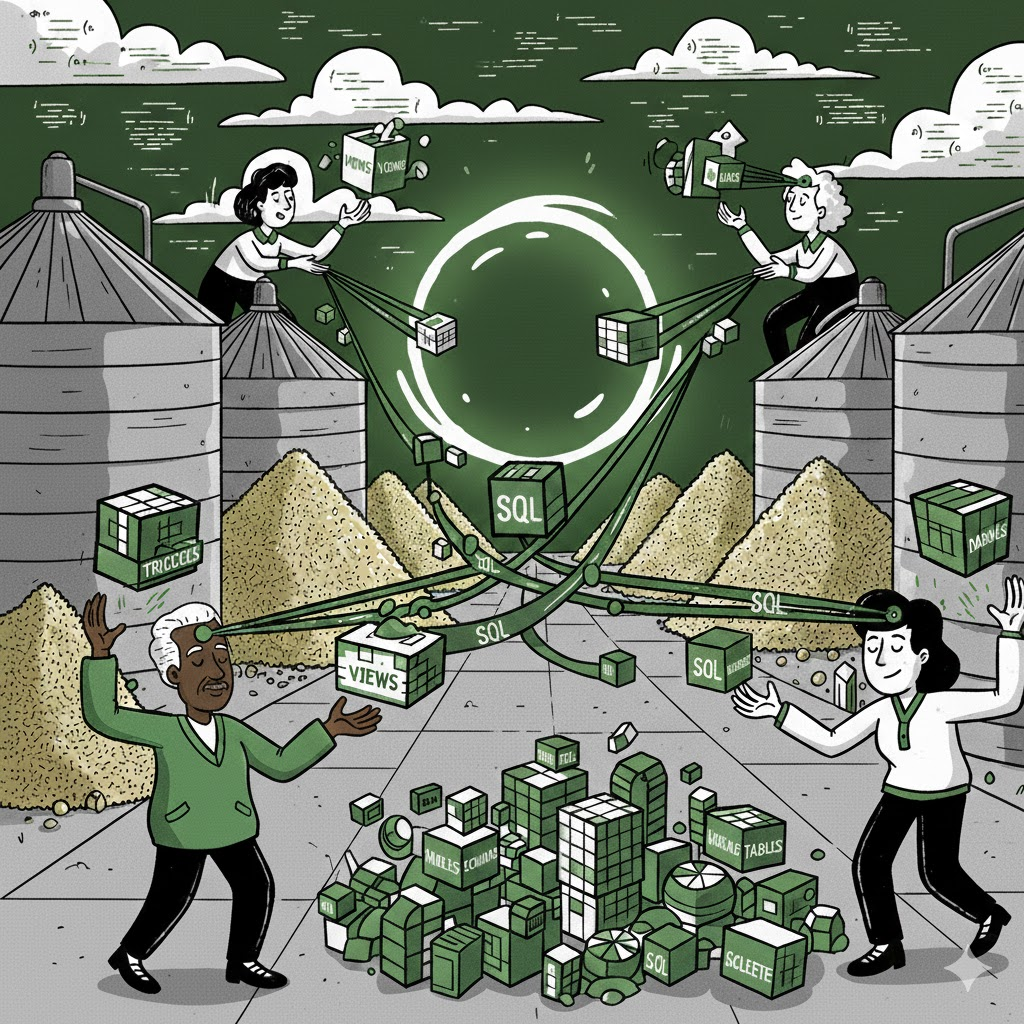
\includegraphics[width= 10cm ]{capa.jpg}}


      \vspace{1.5cm}
      {\Huge\bfseries\color{verdeuni} Capítulo 1 - Conhecendo as ferramentas}

      \vspace{1cm}
      {\Large Universidade de Rio Verde}

    \end{center}

  \end{titlepage}
}
\makecapa
